\label{chpt:results:characterisation of 12 new CVs} % for referencing this chapter elsewhere, use \ref{chpt:label}
\lhead{\emph{Eclipse modelling of 12 CVs}} % This is for the header on each page - perhaps a shortened title

% As previously mentioned, a primary focus of this thesis is to grow the population of eclipse modelled CVs.
A modest backlog of observed CV eclipse light curve data was reduced, calibrated, and modelled, and the results are presented here. All CVs were fit using the new hierarchical model structure described in \S\ref{sect:modelling:optimising eclipse model parameters}, with eclipses binned together where possible, to reduce the complexity of the parameter space. Which specific data were binned together for each system, if any, is given in the tables in \S\ref{sect:observing:observation catalogue}.


\section{Systems chosen for modelling}

The systems modelled here were largely chosen based on their short periods, in an effort to uncover more period-bouncer CVs, as this population is under-sampled in previous eclipse-modelled CVs.
The systems chosen for modelling range in period from $1.4 - 2.2$ hours, and were drawn from a few sources.
The All-Sky Automated Survey for Supernovae (ASASSN) \citep{shappee2014} is sensitive to transients, and is a valuable tool to identify CVs by their outbursts for follow-up once they re-enter quiescence. Such systems are recognised by their ASASSN moniker.
Other candidate systems were gathered from a variety of sources, which are cited below.
% The vsnet alert system also provided several systems, which are marked below with (v).
The modelled systems in this thesis were:
\begin{itemize}
    \setlength\itemsep{0em}
    \item ASASSN-14hq
    \item ASASSN-14kb (a.k.a OGLE-LMC529.30.114)
    \item ASASSN-15pb
    \item ASASSN-17fo
    \item AY For (a.k.a H$\alpha$0242-2802) \citep{woudt2004}
    \item CSS090622 J215636+193242 (hereafter CSS090622) \citep{kato2012,thorstensen2016}
    \item CSS090102 J132536+210037 (hereafter CSS090102) \citep{kato2012}
    \item CSS090419 J162620-125557 (hereafter CSS090419) \citep{kato2012}
    \item MASTER OT J001400.25-561735.0 (hereafter MAS0014) (Woudt, private communication)
    \item OGLE BLG-ECL-000082 (a.k.a BLG510.16.126296, hereafter OGLE82)\todo{Not actually sure where this one came from...}
    \item SDSS J074859.6+312512.7 (hereafter SDSS J0748) \citep{kato2016}
    \item SDSS J152419.33+220920.0 (hereafter SDSS J1524) \citep{southworth2010,michel2013}
\end{itemize}

ASASSN-14hq and ASASSN-15pb were observed by \citet{paterson2019} and had their periods measured, though the observations used in this thesis pre-date this publication.
These two systems were also noted to be in outburst in late 2014 in the case of ASASSN-14hq, and 2015 in the case of ASASSN-15pb.


\section{Results}
\label{sect:results:12 new CVs:results}

All eclipses presented are well-described by their fits, with small residuals. The light curves are contained in Appendix~\ref{appendix:lightcurves}, along with the white dwarf flux distributions and their best-fit white dwarf model atmospheres. The example system of ASASSN-14kb has the lightcurve and flux distribution is shown in Figure~\ref{fig:results:12 new CVs:ASASSN-14kb all lightcurves}, and Figure~\ref{fig:results:12 new CVs:ASASSN-14kb flux plot}, respectively.
In a few cases, the GP appears as a flat line along a residual of 0 despite some obvious scatter, e.g. ASASSN-14hq, seen in Figure~\ref{fig:ASASSN-14hq all lightcurves cont}. This is expected, as in these cases the residuals are fully described by the error in flux and the GP likelihood becomes dominated by the priors, sampling small values of GP amplitude.

None of these systems presented the issues with their characterisations that was seen in Chapter~\ref{chpt:results:three peculiar white dwarfs}. The modelled white dwarf colours were described by cooling tracks well in most cases, with the exceptions of CSS090419 and CSS090622. Spectroscopic follow-up in these cases is desirable to probe these systems more deeply.

Some results are particularly good demonstrations of the ability of the hierarchical GP modelling approach to usefully model poorer quality light curves in tandem with higher quality data.
An example of this is seen in the case of MAS0014, the light curves of which are seen in Figures~\ref{fig:MAS0014 all lightcurves},~\ref{fig:MAS0014 all lightcurves cont 1},~and~\ref{fig:MAS0014 all lightcurves cont 2}, where the high-quality binned data help a subtle bright spot egress to be confidently constrained in the eclipse of 2016/11/07 even in the presence of significant flickering.

A more extreme example is that of SDSS J0748, which has the white dwarf and bright spot ingresses blended together for the majority of observations, but clearly distinct ingresses on the night of 2018/02/05 and somewhat distinct ingresses on 2018/02/07, seen in Figure~\ref{fig:SDSS J0748 all lightcurves}.
Using the hierarchical structure to share information between observations constrains the parameter space, and makes characterisation possible in a system that would otherwise be extremely difficult to model.

Table~\ref{table:12 new cvs:system_parameters} details the physical parameters of these 12 new systems, and notes on the modelling of each is given below.

\begin{figure}
    \centering
    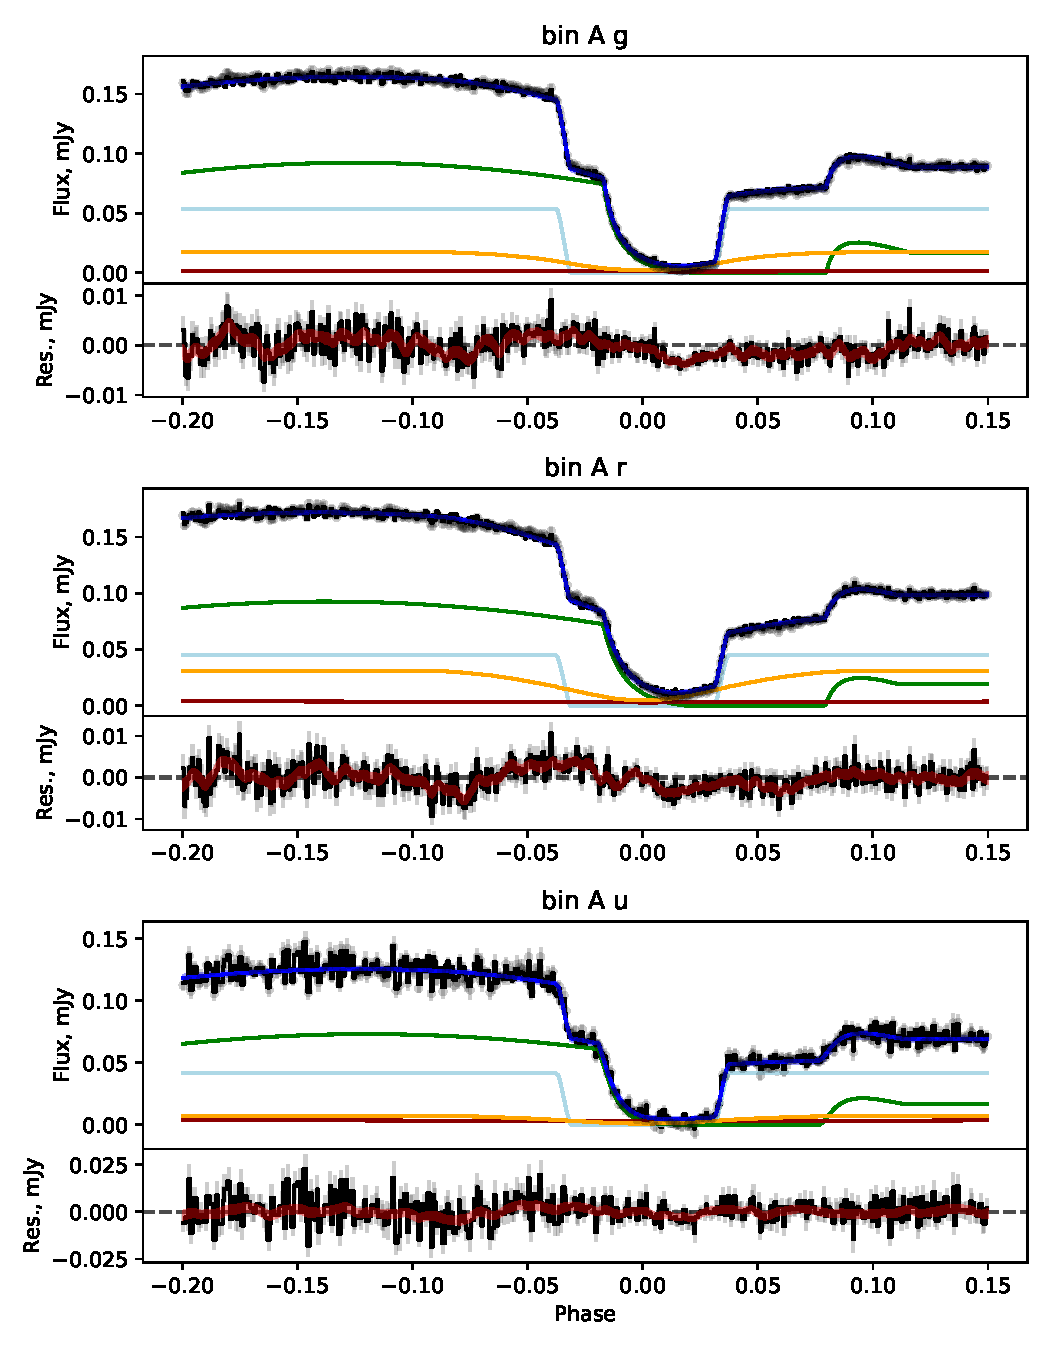
\includegraphics[width=\textwidth]{figures/results/ASASSN-14kb/ASASSN-14kb_ex_1.pdf}
    \caption{Example lightcurve models, of ASASSN-14kb. {\it Top}:~{\bf grey points} are the observed flux, and note that the photometric system is the SDSS as per \S\ref{sect:observations:flux calibrating the lightcurve}; {\bf black line} is the observed flux, with the mean Gaussian process sample subtracted; the {\bf dark blue line} is the mean lightcurve model, and the {\bf blue band} is the standard deviation on this in the MCMC chain. The components of the model are also shown: the {\bf light blue line} is the white dwarf flux, {\bf green line} is the bright spot, {\bf orange line} is the disc, and the {\bf red line} is the donor. {\it Bottom}:~The residuals between the data and model are plotted as the {\bf black line}, with grey error bars. The Gaussian process 1-sigma region is shown as a {\bf red band}.}
    \label{fig:results:12 new CVs:ASASSN-14kb all lightcurves}
\end{figure}
\begin{figure}
    \centering
    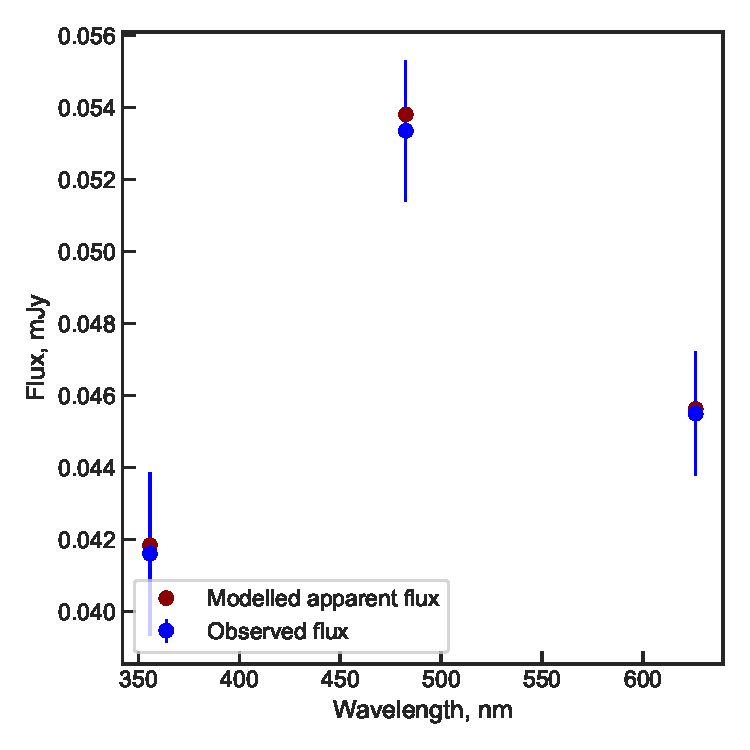
\includegraphics[width=\textwidth]{figures/results/ASASSN-14kb/fluxplot.pdf}
    \caption{The example case of the ASASSN-14kb observed white dwarf fluxes, compared to the best-fit model atmosphere.}
    \label{fig:results:12 new CVs:ASASSN-14kb flux plot}
\end{figure}


\subsection{ASASSN-14hq}

These observations fell into two binning categories. The 2016 and 2017 data were consistent with one another, and the January 2018 data were consistent enough to combine. The eclipse modelling indicates that the disc radius fell in brightness by $\sim 20\%$ in the $g'$ and $\sim 50\%$ in the $u'$ between these two batches, suggesting the disc was in a phase of dumping material onto the white dwarf faster than material enters it from the donor during this period.

For this system, the white dwarf fluxes were well-described by the model cooling tracks, with the white dwarf fitting phase producing a value of $\pi$ that agrees with Gaia ($3.40\pm0.07$ mas and $3.40\pm0.08$ mas, respectively).
Fitting found a somewhat low mass white dwarf, $0.67 \pm 0.07 M_\odot$, though this falls just over $1\sigma$ outside the \citet{pala2020} range of $0.83\pm0.13 M_\odot$ so is well within the expected mass range, and a donor mass of $0.097\pm0.002 M_\odot$, consistent with the `optimal' pre-period minimum CV track.


\subsection{ASASSN-14kb}



\subsection{ASASSN-15pb}


\subsection{ASASSN-17fo}


\subsection{AY For}

AY For had the white dwarf and donor stars' masses estimated spectroscopically in \citet{mason2005} to be $M_{\rm wd} \sim 0.64 M_\odot$ and $M_{\rm donor} \sim 0.17 M_\odot$, with no error reported.
These values are not consistent with my findings of $M_{\rm wd} = 0.78\pm0.02 M_\odot$ and $M_{\rm donor} = 0.106\pm0.006 M_\odot$.
The previous measurement is highly dubious; it is based on inferring a donor mass and radius from the period using the model $M_{\rm donor} - P$ relation presented in \citet{howell2002}, which is then used to calculate a white dwarf mass from a spectroscopic $q$. This relies heavily on a poorly understood relationship, and extrapolates that further when giving a white dwarf mass.
AY For is also claimed by \citet{mason2005} to be a pre-period minimum system, which is corroborated by this more rigorous analysis.

The white dwarf fluxes of AY For were not well-described by the white dwarf cooling tracks, similarly to the systems in \S\ref{sect:three white dwarfs:method WD atmosphere fits}. There is high confidence that this is a real effect rather than a poor calibration, as the field about AY For was observed by the PANSTARRS survey, and the comparison star SDSS magnitudes are reported, which can be used to flux-calibrate the data independently of the standard star method typically used. Comparing these two calibrations finds comparison star fluxes that are within 2\% of each other. Rather, this system possibly suffers from a similar corrupting effect to that seen in the three CVs of Chapter~\ref{chpt:results:three peculiar white dwarfs}, though the disagreement here is not as severe as the extreme case of SSSJ0522-3505. Modelling error is similarly unlikely, as the lightcurve fits generally show distinct ingress and egress features that are replicated in the models. However, based on the in-depth analysis of Chapter~\ref{chpt:results:three peculiar white dwarfs}, we can still consider the system parameters of AY For to be robust.


% Needs reworking
% In addition, the white dwarf fluxes of CSS090419 and CSS090622 appear to significantly brighten in the $i'$ band, seen in Figure~\ref{fig:CSS090419 flux plot} and Figure~\ref{fig:CSS090622 flux plot}, which cannot be described by the white dwarf models used here. However, the disagreement in each case is well within $2 \sigma$, and not seen in the other $i$ band observation, ASASSN-15pb, suggesting this is not a systematic issue. For both systems, the characterisation can still be considered robust.

\subsection{CSS090102}

\subsection{CSS090419}

CSS090419 significantly brightens in the $i'$ band, compared to the $r'$ band. This is unlikely to be calibration error in the $i'$ band, as calibration has otherwise proven to be robust. In addition, this brightening is not seen in the ASASSN-15pb $i'$ band observations, suggesting it is not a systematic issue.

A failure in model optimisation can reasonably be blamed, but can also be eliminated. The resulting fit appears to be acceptable, with little residual flux. These fits are given in Figures~\ref{fig:CSS090419 all lightcurves}~and~\ref{fig:CSS090419 all lightcurves cont 1}.
The white dwarf and bright spot ingresses are somewhat blended in the $r'$ and $i'$, but the egresses are distinct enough to resolve a white dwarf flux. Further, the ingresses in the $u'$ and $g'$ are less blended, allowing the hierarchical structure to use these eclipses to constrain the poor $r'$ and $i'$ data.
These blended features are reflected in large uncertainty in white dwarf flux. Indeed, the standard deviations on all four white dwarf fluxes are large enough that they are consistent with their mean -- a perfectly flat spectrum.

This is not typical white dwarf behaviour, and cannot be reproduced by the white dwarf model atmospheres used here given the constraints. Whilst an extremely hot white dwarf is able to produce a flat spectrum in the optical range, the luminosity of such an object is forbidden by the Gaia distance measurement.
This preference for a flat spectrum is reflected in the high, and highly uncertain, best fit $T_{\rm eff} = 18200 \pm 9000$K, though the posterior $\pi$ distribution is consistent with the Gaia measurement of $1.41\pm0.78$ mas, with slightly reduced uncertainty.
Despite these issues with the white dwarf fitting, as demonstrated in Chapter~\ref{chpt:results:three peculiar white dwarfs} the resulting characterisation can still be considered valid.


\subsection{CSS090622}

\subsection{OGLE82}

\subsection{SDSS J0748}

\subsection{MASOT0014}

\subsection{SDSS J1524}


\newpage

\begin{landscape}

    \begin{table*}
        \centering
        \caption{The system parameters found for the CVs analysed here. The reported parallax, $\pi$, is the posterior distribution from fitting the white dwarf fluxes, c.f.~\S\ref{sect:modelling:fitting white dwarf colours}.}
        \label{table:12 new cvs:system_parameters}
        \begin{tabular}{cccccc}
            \hline \\
            \textbf{System Name:}      & \textbf{ASASSN-14hq}    & \textbf{ASASSN-14kb}     & \textbf{ASASSN-15pb}      & \textbf{ASASSN-17fo}      & \textbf{AY For}       \\
            \hline \hline \\
            $M_\mathrm{WD}/M_\odot$    & $0.67\pm0.01$           & $0.74\pm0.02$            & $0.72\pm0.03$             & $0.85\pm0.01$             & $0.78\pm0.02$         \\
            $R_\mathrm{WD}/R_\odot$    & $0.0119\pm0.0001$       & $0.0113\pm0.0002$        & $0.0115\pm0.0005$         & $0.0099\pm0.0001$         & $0.0106\pm0.0003$ \\
            $M_\mathrm{donor}/M_\odot$ & $0.097\pm0.002$         & $0.134\pm0.003$          & $0.148\pm0.008$           & $0.109\pm0.002$           & $0.106\pm0.006$ \\
            $R_\mathrm{donor}/R_\odot$ & $0.157\pm0.001$         & $0.164\pm0.001$          & $0.210\pm0.004$           & $0.1436\pm0.0007$         & $0.162\pm0.003$ \\
            $q$                        & $0.145\pm0.002$         & $0.182\pm0.002$          & $0.206\pm0.004$           & $0.1267\pm0.0005$         & $0.136\pm0.004$ \\
            \hline
            $P$, hours                 & $1.78384800(7)$         & $1.63453(1)$             & $2.23896(3)$              & $1.477147(2)$             & $1.790756(1)$ \\
            $a/R_\odot$,               & $0.681\pm0.004$         & $0.670\pm0.005$          & $0.824\pm0.014$           & $0.646\pm0.003$           & $0.717\pm0.007$ \\
            $i$                        & $80.35\pm0.06$          & $84.4\pm0.1$             & $79.4\pm0.1$              & $84.23\pm0.03$            & $84.0\pm0.2$ \\
            $K_\mathrm{WD}$, km/s      & $58.0\pm0.9$            & $76.2\pm1$               & $75\pm2$                  & $60.2\pm0.4$              & $57.8\pm2.0$ \\
            $K_\mathrm{donor}$, km/s   & $399\pm2$               & $419\pm3$                & $364\pm6$                 & $468\pm2$                 & $425\pm4$ \\
            \hline
            $\pi$, mas                 & $3.40\pm0.07$           & $2.78\pm0.11$            & $1.0\pm0.2$               & $1.79\pm0.36$             & $2.12\pm0.16$ \\
            $T_{\rm eff}$, K           & $14819\pm800$           & $17700\pm1000$           & $19200\pm1600$            & $14800\pm600$             & $18100\pm500$ \\
            $\log(g), {\rm cgs}$       & $8.11\pm0.02$           & $8.21\pm0.03$            & $8.17\pm0.06$             & $8.37\pm0.02$             & $8.28\pm0.04$ \\
            \hline
            \hline
        \end{tabular}
    \end{table*}

    \begin{table*}
        \centering
        \caption{Table~\ref{table:12 new cvs:system_parameters}, continued.}
        \label{table:12 new cvs:system_parameters cont 1}
        \begin{tabular}{cccccc}
            \hline \\
            \textbf{System Name:}      & \textbf{CSS090102}     & \textbf{CSS090419}    & \textbf{CSS090622}    & \textbf{OGLE82}   & \textbf{SDSS J0748} \\
            \hline \hline \\
            $M_\mathrm{WD}/M_\odot$    & $0.62\pm0.03$          & $0.59\pm0.08$         & $0.67\pm0.06$         & $0.83\pm0.01$     & $0.68\pm0.02$ \\
            $R_\mathrm{WD}/R_\odot$    & $0.0126\pm0.0004$      & $0.0122\pm0.0009$     & $0.0112\pm0.0007$     & $0.0099\pm0.0002$ & $0.0121\pm0.0004$ \\
            $M_\mathrm{donor}/M_\odot$ & $0.060\pm0.003$        & $0.087\pm0.011$       & $0.104\pm0.009$       & $0.131\pm0.004$   & $0.066\pm0.004$ \\
            $R_\mathrm{donor}/R_\odot$ & $0.119\pm0.002$        & $0.152\pm0.007$       & $0.155\pm0.005$       & $0.170\pm0.002$   & $0.117\pm0.002$ \\
            $q$                        & $0.094\pm0.002$        & $0.146\pm0.003$       & $0.159\pm0.008$       & $0.157\pm0.002$   & $0.095\pm0.004$ \\
            \hline
            $P$, hours                 & $1.49723786(5)$        & $1.81062621(6)$       & $1.702302(6)$         & $1.7263398(6)$    & $1.39947(1)$ \\
            $a/R_\odot$,               & $0.582\pm0.008$        & $0.660\pm0.030$       & $0.661\pm0.020$       & $0.720\pm0.006$   & $0.575\pm0.007$ \\
            $i$                        & $88.7\pm0.6$           & $80.9\pm0.1$          & $88.2\pm0.6$          & $83.9\pm0.1$      & $81.7\pm0.2$ \\
            $K_\mathrm{WD}$, km/s      & $40.9\pm1.2$           & $56.0\pm2.7$          & $63.7\pm2.5$          & $68.5\pm1.0$      & $42.2\pm1.8$ \\
            $K_\mathrm{donor}$, km/s   & $431\pm6$              & $381\pm16$            & $408\pm12$            & $435\pm3$         & $450\pm5$ \\
            \hline
            $\pi$, mas                 & $1.41\pm0.30$          & $1.42\pm0.69$         & $2.02\pm0.27$         & $3.82\pm0.12$     & $1.83\pm0.14$ \\
            $T_{\rm eff}$, K           & $14800\pm1200$         & $18200\pm9000$        & $9800\pm1500$         & $18000\pm4000$    & $22500\pm3000$ \\
            $\log(g), {\rm cgs}$       & $8.00\pm0.33$          & $8.04\pm0.12$         & $8.16\pm0.08$         & $8.37\pm0.03$     & $8.11\pm0.03$ \\
            \hline
            \hline
        \end{tabular}
    \end{table*}

    \begin{table*}
        \centering
        \caption{Table~\ref{table:12 new cvs:system_parameters}, continued.}
        \label{table:12 new cvs:system_parameters cont 2}
        \begin{tabular}{ccc}
            \hline \\
            \textbf{System Name:}      & \textbf{MASOT0014}     & \textbf{SDSS J1524} \\
            \hline \hline \\
            $M_\mathrm{WD}/M_\odot$    & $0.86\pm0.03$          & $0.80\pm0.04$ \\
            $R_\mathrm{WD}/R_\odot$    & $0.0097\pm0.0003$      & $0.0103\pm0.0005$ \\
            $M_\mathrm{donor}/M_\odot$ & $0.122\pm0.007$        & $0.074\pm0.008$ \\
            $R_\mathrm{donor}/R_\odot$ & $0.165\pm0.003$        & $0.132\pm0.005$ \\
            $q$                        & $0.142\pm0.004$        & $0.093\pm0.007$ \\
            \hline
            $P$, hours                 & $1.7167077(5)$         & $1.56764953(2)$ \\
            $a/R_\odot$,               & $0.722\pm0.008$        & $0.652\pm0.01197$ \\
            $i$                        & $84.8\pm0.3$           & $86.7\pm1.1$ \\
            $K_\mathrm{WD}$, km/s      & $63.2\pm2.0$           & $42.9\pm3.4$ \\
            $K_\mathrm{donor}$, km/s   & $445\pm5$              & $461\pm7$ \\
            \hline
            $\pi$, mas                 & $2.42\pm0.11$          & $1.92\pm0.19$ \\
            $T_{\rm eff}$, K           & $17300\pm1000$         & $12500\pm1100$ \\
            $\log(g), {\rm cgs}$       & $8.37\pm0.04$          & $8.32\pm0.06$ \\
            \hline
            \hline
        \end{tabular}
    \end{table*}
\end{landscape}



\section{Exploration of results}
\label{sect:discussion:eclipse modelling of 12 CVs}

The observed donor properties can be compared to the \citet{knigge11}-like MESA donor tracks. Figure~\ref{fig:discussion:donor model with eclipsers plotted} shows the full sample of short-period eclipse modelled CVs (a catalogue of these systems is given in Appendix~\ref{appendix:eclipse modelled CV data tables}) plotted with the `standard' donor track that includes only gravitational braking below the gap and the disagreement between model and data indeed persists. Whilst there is a large scatter present, new data continue to lie systematically to the right of the `standard' model track, and the need for extra AML continues to be supported by observations.\todo{The K11 mass-radius relation could be updated? Not really worth it, not my focus and not that many new systems.}
\begin{figure}
    \centering
    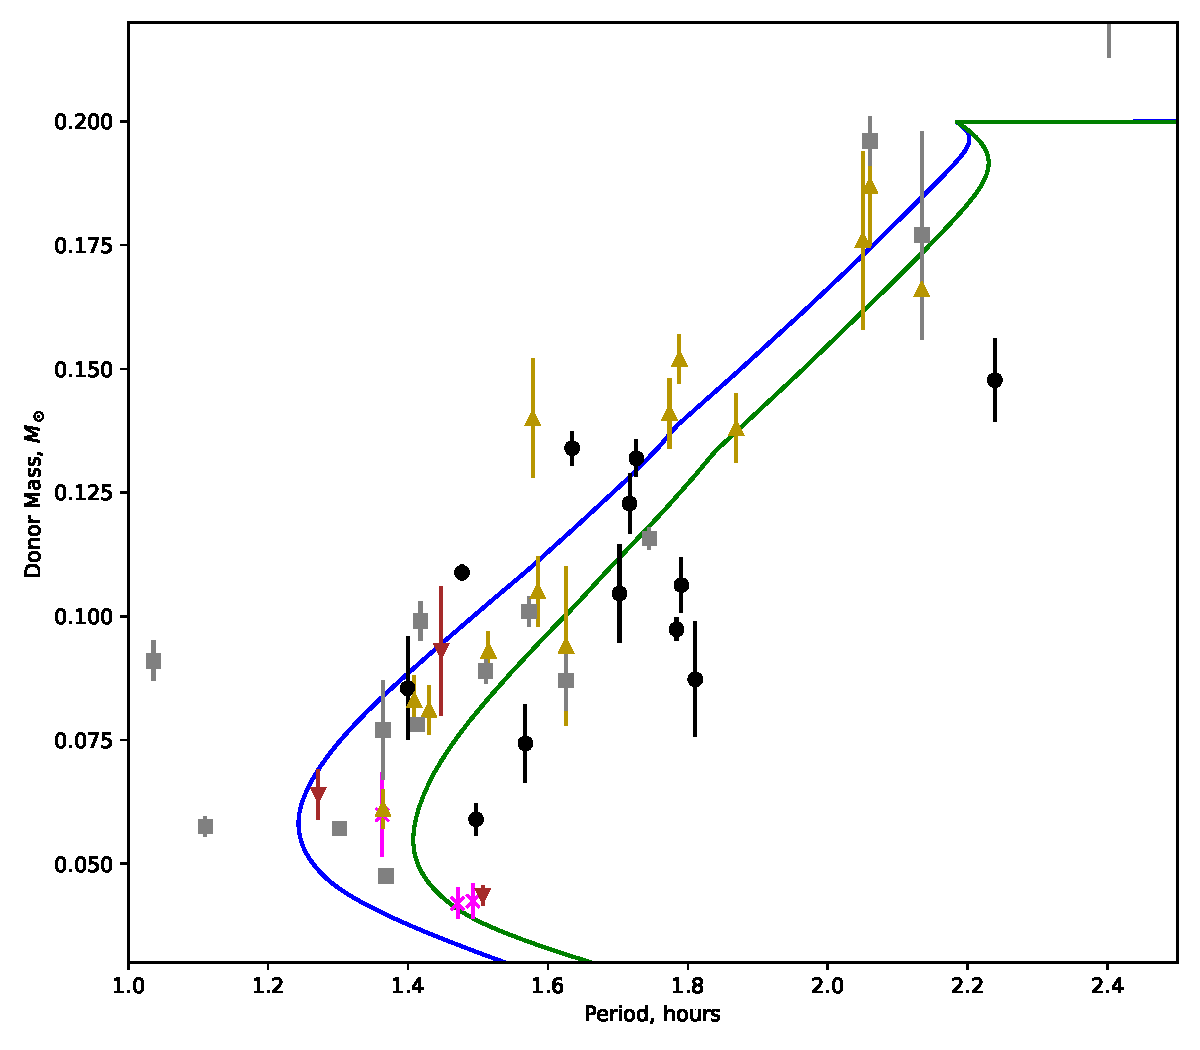
\includegraphics[width=\textwidth]{figures/results/Mdot/K11_donor_track_with_eclipse_modelled_data.pdf}
    \caption{Showing how eclipse modelled observations compare with evolutionary models in the short period regime. The {\bf solid blue line} is the `standard' MESA CV donor track, and the {\bf solid green line} is the `optimal' track, described in \S\ref{sect:results:reproducing K11 tracks}. The {\bf black data with errors} are observations: {\bf crosses} are the 3 CVs with peculiar colours from Chapter~\ref{chpt:results:three peculiar white dwarfs}, {\bf circles} are the 12 systems of Chapter~\ref{chpt:results:characterisation of 12 new CVs}, {\bf upright triangles} are data from \citet{McAllister2019}, {\bf squares} are from \citet{Savoury2011}, and the {\bf inverted triangles} are the supplementary systems from \citet{copperwheat2010,mcallister2015,mcallister2017,mcallister2017b}.}
    \label{fig:discussion:donor model with eclipsers plotted}
\end{figure}



\subsection{A preliminary look at AML in CVs}
\label{sect:discussion AML}

The published results and analysis of the three CVs in Chapter~\ref{chpt:results:three peculiar white dwarfs} \citep{wild2021} pre-dates the more fully developed method to infer a donor mass loss rate described in \S\ref{sect:modelling:optimising mass loss rate to observations}.
That analysis method was repeated using the new data presented here, significantly increasing the population of well-characterised CVs compared to what was available at publication. The core findings of that work persist with the new data set, lending further credence to the results.

In order to qualitatively evaluate missing AML, the period \textit{excess} was examined, $P_{\rm ex} = P_{\rm obs} - P_{\rm std}$. Here, $P_{\rm obs}$ is the observed period, and $P_{\rm std}$ is the period predicted by the MESA CV donor track with only $1\times$ gravitational braking below the period gap, interpolated across $M_{\rm donor}$.
To determine $P_{\rm ex}$ from a measured $(P_{\rm obs}, M_{\rm donor})$ pair, mass samples are drawn from the modelled posterior distribution of $M_{\rm donor}$, and period is interpolated at each mass from the evolutionary tracks to give a corresponding $P_{\rm std}$ distribution. As $P_{\rm std}$ is very sensitive to $M_{\rm donor}$, the $P_{\rm std}$ error dominates the uncertainty in $P_{\rm ex}$.
A positive $P_{\rm ex}$ indicates that the model is missing AML, and a negative $P_{\rm ex}$ indicates a model that has too much AML, relative to an observation.

The validity of $P_{\rm ex}$ is vulnerable to two key systematic biases; the validity of $P_{\rm std}$ (itself contingent on the accuracy of a variety of model assumptions and biases), and the inherent physical variation of the CV population. This is the secondary motivation for the development of the more rigorous methodology of \S\ref{sect:modelling:optimising mass loss rate to observations}, after the primary motivation of trying to improve on the qualitative nature of the $P_{\rm ex}$ approach.

CVs may follow inherently different evolutionary tracks due to differences in donor metallicity \citep{stehle1997, harrison2016}, white dwarf mass \citep{knigge2006}, and the age of the donor when it first contacts the Roche lobe \citep{howell2001}. A population-wide scatter in this parameter space is not captured in the \citet{knigge11} model, which uses fixed values for these variables, but justification for the adopted values are given \citep{knigge11, knigge2006}.
If any individual system deviates from the adopted values in the models of \citet{knigge11} then $P_{\rm ex}$ for that system will be influenced by these differences as well as any extra AML. However, conclusions about $P_{\rm ex}$ drawn from the population at large should remain robust, as long as the population doesn't differ systematically from the values adopted in the models.
The white dwarf mass used by \citet{knigge11} is somewhat lower than more recent observations suggest, using $M_{\rm WD} = 0.75 M_\odot$ versus the more recent value of $M_{\rm WD} = 0.83 \pm 0.17 M_\odot$ \citep{pala2020}.\todo{I can re-do this with MESA, but I really don't think it's worth bothering...}
An updated version of Knigge's modelling is necessary to properly characterise the effect of this change on the donor evolutionary tracks, as this will affect both the size of the Roche lobes, and the rate of gravitational wave AML; alternatively, MESA models could be used here, though these are subject to their own biases and assumptions.
Other CV models suggest that the effect of correcting $M_{\rm wd}$ will be small, at most around 2 minutes \citep{goliasch2015}. This analysis is not rigorous enough for this to become an issue, and the effects of using an incorrect white dwarf mass is considered acceptable.

More seriously, $P_{\rm ex}$ is only an accurate proxy of additional AML if the underlying donor physics in the model are correct. For example, if the models incorrectly predict the mass of systems in the period gap, this can have a large effect on $P_{\rm ex}$. In the models of \citet{knigge11} this mass is fixed at the empirically derived value of $0.2 M_\odot$, as observations of superhumping and eclipsing CVs suggest that period gap occurs at donor masses of $0.20 \pm 0.02 M_\odot$ \citep{knigge2006}. Using model tracks with lower or higher masses for the donor mass of the period gap would alter $P_{\rm ex}$, though in this case the broad trend in $P_{\rm ex}$ will again be unchanged.

The result is plotted in Figure~\ref{fig:period excess}. These data are fit with a straight line, and as the data have significant uncertainty in both axes, the sum orthogonal distance (weighted by uncertainty) from the data is minimised to find the best fit \citep{hogg2010}. Python's \lstinline{SciPy} package, \lstinline{ODR} was used to perform this fitting.

 The best-fit lines to the two data sets are $P_{\rm ex} = -(11.8\pm3.7) M_{\rm donor} + (1.3\pm0.4)$ and $P_{\rm ex} = -(2.0\pm0.4) M_{\rm wd} + (1.6\pm0.3)$.
I find that the best-fit to $P_{\rm ex}$ as a function of both $M_{\rm donor}$ and $M_{\rm wd}$ to be significant: $5\sigma$ from the null hypothesis of 0 in the case of $M_{\rm wd}$, and $\sim 3\sigma$ for $M_{\rm donor}$.
 However, note that the best-fit line for $M_{\rm donor}$ does \textit{not} pass through $P_{\rm ex} = 0$ at $M_{\rm donor} = 0.20 M_\odot$ as expected, unless the $3\sigma$ confidence on the gradient and intercept are considered.

Again, it is stressed that the only robust product of this analysis is the \textit{sign of the gradient} of the $M - P_{\rm ex}$ relationship, and that its steepness and y-intercept are both subject to systematic errors that are not captured in the statistical errors given above. Despite this, the clear and statistically significant increase in $P_{\rm ex}$ towards low masses implies that additional AML has a larger effect on the donor at low masses.

Note that $P_{\rm ex}$ considers a changing gravitational braking strength, which declines as the total system mass falls.
There are then three cases to describe the trend in $P_{\rm ex}$: the excess AML also declines in strength but more slowly than gravitational losses; excess AML is roughly constant across the range of $M_{\rm donor}$ or $M_{\rm wd}$; or excess AML actually increases in strength towards lower $M_{\rm donor}$ or $M_{\rm wd}$. Note that none of these options translate to the ``optimal'' \citet{knigge11} models which adopt additional AML of the same form as GWB, but are compatible with the eCAML solution for excess AML.


\begin{figure}
    \centering
    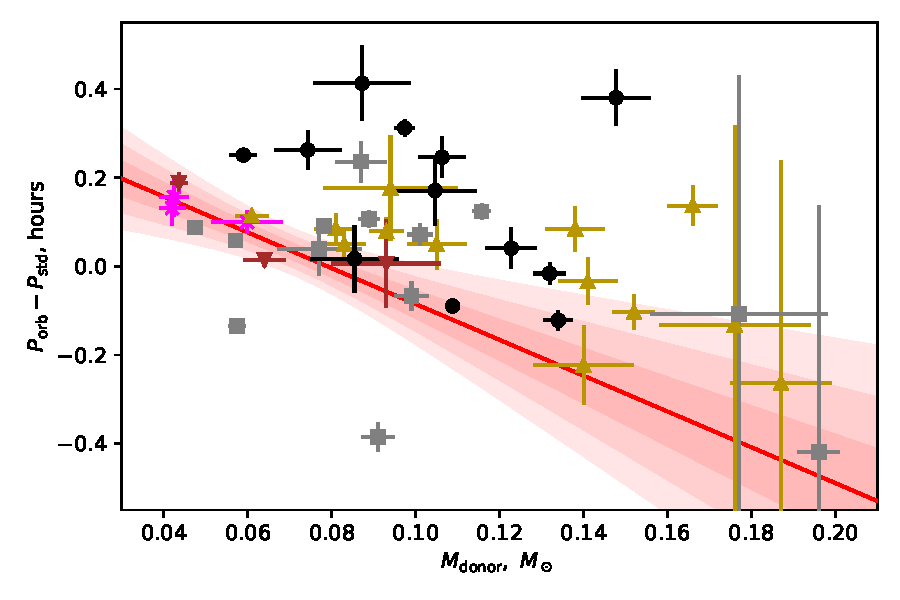
\includegraphics[width=\columnwidth]{figures/results/Mdot/Period_excess_Mr.pdf}
    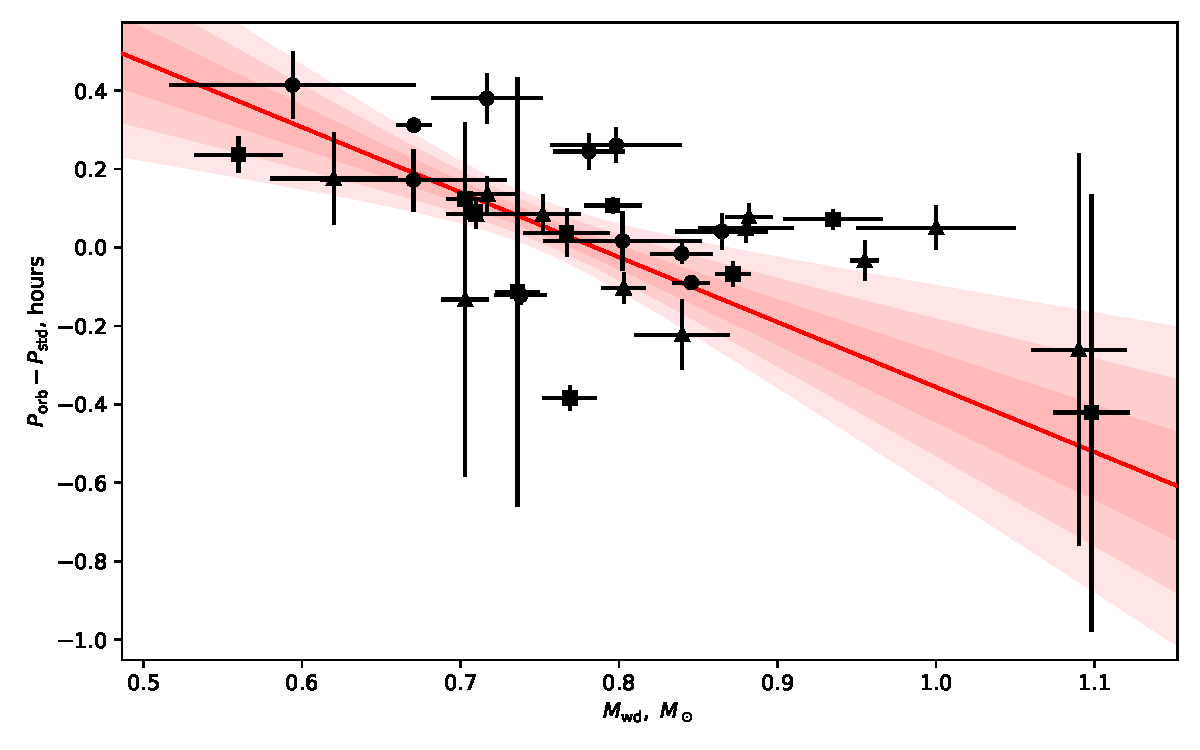
\includegraphics[width=\columnwidth]{figures/results/Mdot/Period_excess_Mwd.pdf}
    \caption{The relation between the two body masses, and the period excess, $P_{\rm ex}$ is shown. The {\bf black crosses with error bars} are the observed data, and the {\bf solid red line} shows the best-fit solution to the data. {\bf Shaded red regions} show successively lower confidence intervals, with the darkest region being $1\sigma$ confidence, and the lightest region being $3\sigma$ confidence. The lines of best fit have the forms: $P_{\rm ex} = -(11.8\pm3.7) M_{\rm donor} + (1.3\pm0.4)$ and $P_{\rm ex} = -(2.0\pm0.4) M_{\rm wd} + (1.6\pm0.3)$.}
    \label{fig:period excess}
\end{figure}
% \begin{figure}
%     \centering
%     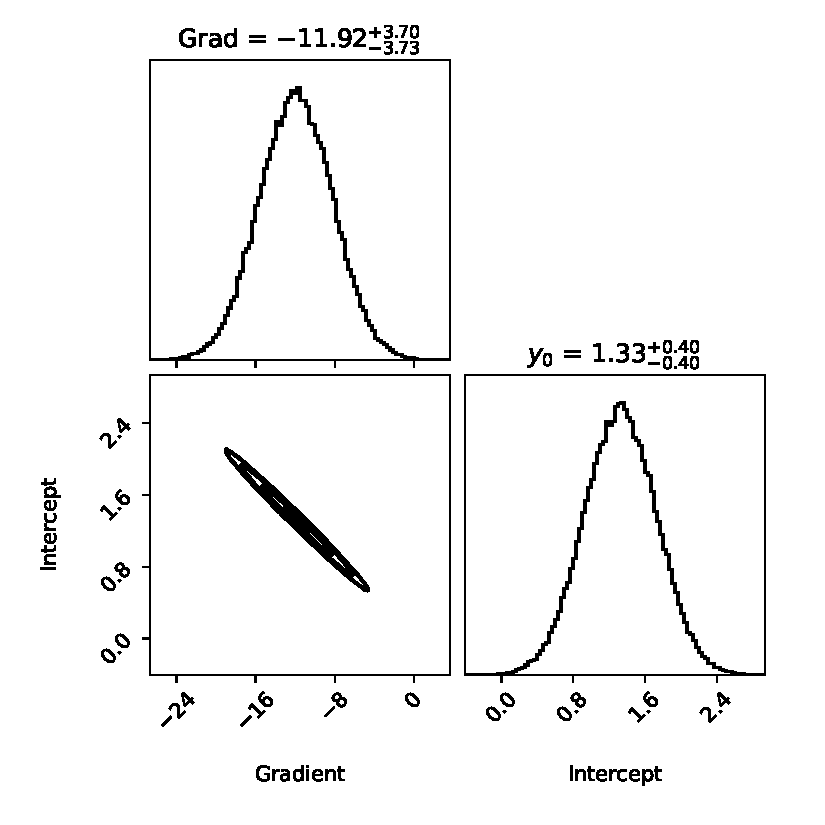
\includegraphics[width=\columnwidth]{figures/results/Mdot/Period_excess_Mr_corner.pdf}
%     \caption{Showing the distribution of the best fit to the $M_{\rm donor} - P_{\rm ex}$ relationship plotted in the top panel of Figure~\ref{fig:period excess}.}
%     \label{fig:period excess donor_corner}
% \end{figure}
% \begin{figure}
%     \centering
%     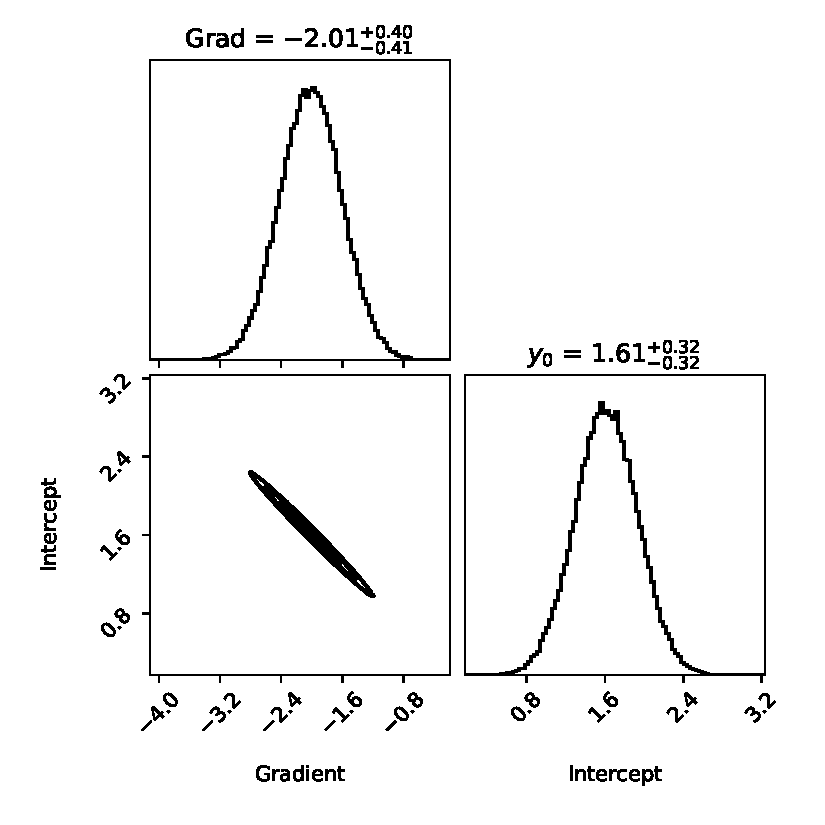
\includegraphics[width=\columnwidth]{figures/results/Mdot/Period_excess_Mwd_corner.pdf}
%     \caption{Showing the distribution of the best fit to the $M_{\rm wd} - P_{\rm ex}$ relationship plotted in the bottom panel of Figure~\ref{fig:period excess}.}
%     \label{fig:period excess white dwarf corner}
% \end{figure}
